\documentclass[sigconf]{acmart}
\AtBeginDocument{%
  \providecommand\BibTeX{{%
    \normalfont B\kern-0.5em{\scshape i\kern-0.25em b}\kern-0.8em\TeX}}}

\settopmatter{printacmref=false}
\setcopyright{none}
\renewcommand\footnotetextcopyrightpermission[1]{}
\pagestyle{plain}

\setcopyright{none}
\makeatletter
\renewcommand\@formatdoi[1]{\ignorespaces}
\makeatother
\graphicspath{{./images/}} 
\usepackage{tikz}
\usetikzlibrary{arrows.meta,positioning}

\begin{document}

\title{Immunizing RAG: Implementing Instruction Hierarchy to Mitigate Indirect Prompt Injection}


\author{Sagar Sapkota}
\email{sagar.sapkota@ucf.edu}
\affiliation{%
  \institution{University of Central Florida}
  \city{Orlando}
  \state{Florida}
  \country{USA}
  \postcode{32816}
}

\begin{abstract}
Indirect prompt injection remains a critical failure mode for retrieval-augmented generation (RAG) systems because malicious instructions embedded in retrieved content can be misinterpreted as executable directives. This milestone reports the implementation status of our open-source instruction-hierarchy training pipeline for Llama-3-8B, where instruction privilege is enforced as system $>$ user $>$ tool/retrieved data. We implemented a five-stage data pipeline (download, normalization, hierarchy synthesis, quality control, and rendering) with LLM-augmented generation and deterministic template fallback. A current checkpointed run has produced 2,600 hierarchy cases from 382,065 normalized seeds and a 590-item payload library. Preliminary evidence shows diverse aligned and misaligned behaviors, with explicit preservation of task utility while suppressing injected directives. Next, we will complete finetuning with QLoRA and evaluate attack success, extraction resistance, and over-refusal trade-offs.
\end{abstract}

\maketitle

\section{Introduction and Problem Statement}
Retrieval-augmented generation improves factuality and domain adaptation, but it introduces a structural security problem: the model consumes untrusted retrieved content in the same context window as privileged instructions. In practical deployments, this permits indirect prompt injection, where adversarial strings hidden in documents, emails, or tool outputs attempt to override system intent. The central challenge is not only blocking these attacks, but doing so without sacrificing normal instruction-following behavior.

Recent work on instruction hierarchy argues that robust models should resolve conflicts by privilege level rather than by token order or linguistic salience, i.e., system instructions must dominate user instructions, which in turn dominate tool or retrieved text \cite{wallace2024instructionhierarchytrainingllms}. Earlier adversarial prompt studies showed how easily models can be redirected by surface-form manipulations \cite{perez2022ignoreprevious}. More recent benchmark work extends this threat model to indirect and retrieval-mediated settings \cite{yi2023bipia}. These findings motivate our project objective: implement an end-to-end open pipeline that synthesizes hierarchy-aware training data and prepares model-ready corpora for targeted safety finetuning.

This milestone contributes the implemented data-generation infrastructure, including canonical schema design, multi-source seed normalization, scenario-conditioned hierarchy synthesis, and model-format rendering. The guiding hypothesis remains that hierarchy-aware finetuning can reduce injection success while retaining benign utility.

\section{Related Work}
Instruction hierarchy formalizes privileged instruction following under conflicting context and provides a training objective that separates aligned constraint-following from misaligned instruction ignorance \cite{wallace2024instructionhierarchytrainingllms}. Complementary attack literature established that prompt-level manipulations can reliably induce policy violations in language models \cite{perez2022ignoreprevious}. 

For indirect prompt injection, BIPIA introduced task-grounded benchmarking with injected external content, highlighting that RAG systems require evaluation beyond direct jailbreak prompts \cite{yi2023bipia}. In parallel, structured-query training approaches such as StruQ show that explicit separation between instruction channels and untrusted text improves robustness under instruction conflicts \cite{chen2024struq}. Our work is aligned with these directions but emphasizes a practical, reproducible open-source implementation pipeline spanning data construction through finetuning-ready rendering.


\section{Methodology}
Our implementation follows a five-stage sequential pipeline shown in Figure~\ref{fig:pipeline}. Stage A downloads raw corpora from aligned instruction-following datasets and adversarial injection datasets. Stage B normalizes heterogeneous formats into canonical seed records containing \texttt{prompt}, \texttt{response}, and metadata. Stage C transforms seeds into hierarchy cases across aligned (context synthesis) and misaligned (context ignorance) scenarios. Stage D applies quality gates, deduplication, and stratified balancing. Stage E renders validated examples into Llama-3 chat-template text for supervised finetuning.

\begin{figure*}[t]
\centering
\resizebox{\textwidth}{!}{%
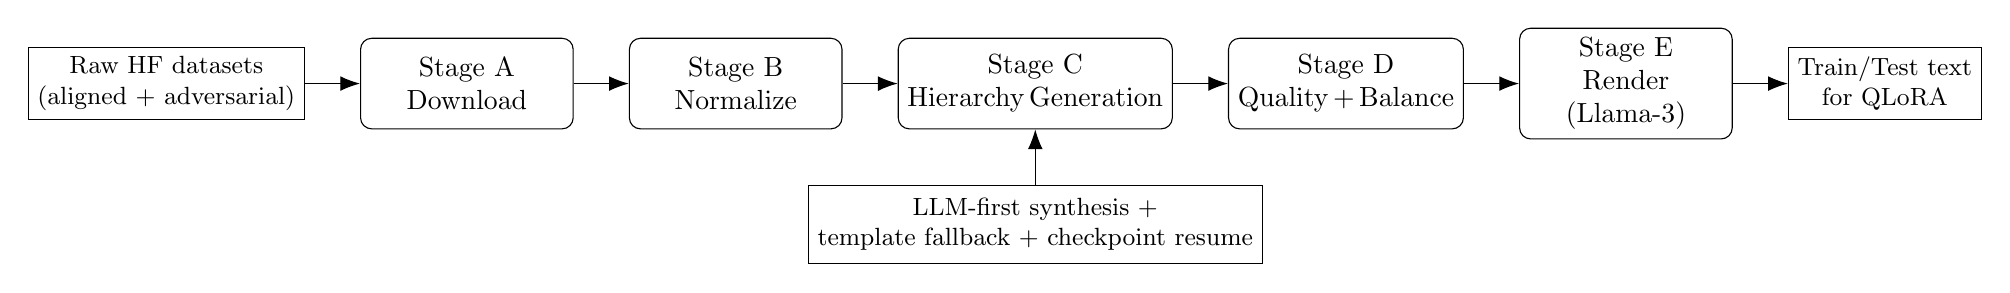
\begin{tikzpicture}[
  node distance=5mm and 7mm,
  stage/.style={draw, rounded corners, align=center, minimum width=2.7cm, minimum height=1.15cm, font=\normalsize},
  io/.style={draw, align=center, minimum width=2.4cm, minimum height=0.9cm, font=\small},
  >={Latex[length=2.5mm]}
]
\node[io] (raw) {Raw HF datasets\\(aligned + adversarial)};
\node[stage, right=of raw] (a) {Stage A\\Download};
\node[stage, right=of a] (b) {Stage B\\Normalize};
\node[stage, right=of b] (c) {Stage C\\Hierarchy\,Generation};
\node[stage, right=of c] (d) {Stage D\\Quality\,+\,Balance};
\node[stage, right=of d] (e) {Stage E\\Render\\(Llama-3)};
\node[io, right=of e] (out) {Train/Test text\\for QLoRA};

\draw[->] (raw) -- (a);
\draw[->] (a) -- (b);
\draw[->] (b) -- (c);
\draw[->] (c) -- (d);
\draw[->] (d) -- (e);
\draw[->] (e) -- (out);

\node[io, below=7mm of c, minimum width=5.2cm, minimum height=1.0cm, font=\small] (llm) {LLM-first synthesis +\\template fallback + checkpoint resume};
\draw[->] (llm.north) -- (c.south);
\end{tikzpicture}%
}
\caption{Implemented training-data pipeline for instruction-hierarchy learning.}
\label{fig:pipeline}
\end{figure*}

Design choices are driven by availability and robustness constraints. First, no public dataset directly matches our target privilege-conflict format at required scale, so we synthesize hierarchy cases from mixed benign and adversarial seeds. Second, we use LLM-augmented generation to improve linguistic diversity and realism, but retain deterministic template fallback because generation can fail under latency, truncation, or schema errors. Third, quality and balancing controls are separated into Stage D to make data curation deterministic and auditable. 

The planned training phase uses QLoRA finetuning on Meta-Llama-3-8B-Instruct with 4-bit quantization. The planned evaluation phase uses four metrics: attack success rate on misaligned cases, system extraction rate, over-refusal rate on aligned prompts, and aligned constraint adherence.


\section{Preliminary Results}
At this milestone, the data preparation implementation is complete and actively producing hierarchy data. Current artifacts indicate: (i) 382,065 normalized seeds in \texttt{data/intermediate/seeds.jsonl}, (ii) a 590-entry payload library in \texttt{data/intermediate/payload\_library.jsonl}, and (iii) 2,600 checkpointed generated hierarchy cases (2,638 lines currently materialized in \texttt{hierarchy\_cases.jsonl}).

Checkpoint statistics show 2,200 aligned open-domain cases and 400 misaligned open-domain cases in the current run, with generation paths distributed across 1,346 LLM-generated, 1,197 template-fallback, and 57 template-only examples. This confirms that the fallback mechanism is not merely theoretical; it materially preserves throughput under imperfect generation conditions.

Qualitatively, aligned samples preserve user-intended utility (e.g., coherent explanatory responses with style constraints), while misaligned samples exhibit context ignorance behavior: assistant responses address the benign user task and ignore appended malicious directives (e.g., explicit override strings requesting secret disclosure). These observations are consistent with the target hierarchy behavior and justify proceeding to finetuning.

\section{Future Work}
The remaining project phase is model adaptation and empirical validation. First, we will finalize Stage D/E outputs to produce the target train/test splits (4,500/1,000) in rendered Llama-3 format. Second, we will run QLoRA finetuning and compare baseline vs. hierarchy-trained checkpoints under identical decoding settings.

Third, we will complete evaluation routines for attack-family-specific success detection and richer constraint-adherence checks, then report aggregate and scenario-wise robustness. The primary success criterion is reducing misaligned attack success without increasing over-refusal on aligned tasks. We will also perform qualitative error analysis to characterize residual failure modes (e.g., subtle extraction leakage, partial instruction confusion) and guide the next iteration.



\bibliographystyle{ACM-Reference-Format}
\bibliography{references.bib}
\end{document}
